\documentclass[11pt,a4paper]{article}

% --- packages ---------------------------------------------------------------
\usepackage[utf8]{inputenc}
\usepackage[T1]{fontenc}
\usepackage[a4paper,margin=2.5cm]{geometry}
\usepackage{amsmath,amssymb}
\usepackage{graphicx}
\usepackage{booktabs}
\usepackage{caption}
\usepackage{subcaption}
\usepackage{xcolor}
\usepackage[colorlinks=true,linkcolor=black,citecolor=black,urlcolor=blue]{hyperref}

\graphicspath{{../results/figures/}}
\captionsetup{font=small}

% --- title ------------------------------------------------------------------
\title{\textbf{Density Estimation Showdown:\\
A Controlled Comparison of Parzen Windows, $k$-NN,\\
Gaussian Mixtures, and the Parzen Neural Network}}

\author{
Leonid Vasilev (163880) \and
Akbar Hasanov (167789) \and
Basel Altamimi (169559)
}
\date{
Artificial Intelligence, A.Y. 2025/2026 --- Prof.\ Edmondo Trentin\\
MSc in Artificial Intelligence and Automation Engineering, University of Siena\\[4pt]
\today
}

\begin{document}
\maketitle

\begin{abstract}
We present a reduced-scale empirical study comparing four probability density
estimation methods: the Parzen window (kernel density estimation), $k$-nearest
neighbour ($k$-NN) density estimation, the Gaussian Mixture Model (GMM) fitted
by Expectation--Maximization, and the Parzen Neural Network (PNN) of Trentin and
Gori. The Parzen, $k$-NN and PNN estimators are implemented from scratch. We
evaluate on synthetic Gaussian-mixture data, where the true density is known and
the Integrated Squared Error (ISE) can be measured, and on the real Old Faithful
geyser benchmark, evaluated by held-out log-likelihood. Across 20 random seeds
and 10-fold cross-validation we find that the GMM is the most accurate (its
parametric assumption matches the data), while the PNN reproduces the Parzen
estimate almost exactly (ISE $0.0032$ vs.\ $0.0033$; on Old Faithful the
PNN--Parzen difference is \emph{not} statistically significant, Holm-adjusted
Wilcoxon $p=0.32$) yet evaluates a query in roughly constant time, about
$300\times$ faster than Parzen at $N=5000$. We confirm all conclusions with
Wilcoxon signed-rank tests under Holm correction, and we ablate the PNN's
unit-integral soft constraint, showing it restores probabilistic validity
(integral $1.045\!\rightarrow\!1.007$) at no measurable accuracy cost.
\end{abstract}

% ============================================================================
\section{Introduction}
% ============================================================================
Probability density estimation is the unsupervised problem of recovering the
density $p(\mathbf{x})$ that generated a sample
$\{\mathbf{x}_i\}_{i=1}^N \subset \mathbb{R}^d$. It underpins classification
(through Bayes' rule), novelty detection, and generative modelling. The classical
methods trade off in characteristic ways: \emph{non-parametric} estimators
(Parzen windows, $k$-NN) make few assumptions but store the entire training set
and are slow at query time; \emph{parametric} estimators (the GMM) are compact
and fast but biased when their assumed form is wrong.

This project studies a fourth option that sits between these regimes: the
\textbf{Parzen Neural Network} (PNN) of Trentin and Gori~\cite{trentin2001parzen},
a small multilayer perceptron trained by regression to reproduce the Parzen
estimate. Once trained it is a compact function evaluated in a single forward
pass, independent of $N$. A plain network output is not a valid density, so
following Trentin's later work on soft-constrained networks satisfying the
Kolmogorov axioms~\cite{trentin2018soft} we enforce non-negativity through the
output head and push the integral of the learned density towards one with a soft
penalty.

Our contributions are: (i) clean, from-scratch implementations of Parzen, $k$-NN
and the PNN behind a common interface, validated against reference
implementations; (ii) a controlled comparison on synthetic and real data using
ISE and held-out log-likelihood; (iii) a query-time scalability study; (iv) a
statistical analysis (Wilcoxon signed-rank with Holm correction); and (v) an
ablation of the PNN's unit-integral constraint. The full pipeline is
reproducible from a single random seed.

% ============================================================================
\section{Methods}
% ============================================================================
All estimators share one interface: \texttt{fit}, \texttt{score\_samples}
returning $p(\mathbf{x})$ in linear space, and \texttt{log\_likelihood}
returning the mean $\log p(\mathbf{x})$.

\subsection{Parzen window (kernel density estimation)}
With an isotropic (or diagonal) Gaussian kernel of bandwidth $\mathbf{h}$,
\begin{equation}
\hat p_{\text{Parzen}}(\mathbf{x})
= \frac{1}{N}\sum_{i=1}^{N}
\frac{1}{(2\pi)^{d/2}\prod_j h_j}
\exp\!\left(-\tfrac12 \sum_{j=1}^{d}\frac{(x_j - x_{ij})^2}{h_j^2}\right).
\label{eq:parzen}
\end{equation}
The bandwidth is a first-class experimental variable. We default to Silverman's
rule of thumb, $h_j = \sigma_j\,(4/((d+2)N))^{1/(d+4)}$~\cite{silverman1986}, and
also provide $k$-fold cross-validated selection that maximises held-out
log-likelihood. Equation~\eqref{eq:parzen} is evaluated with a numerically
stable log-sum-exp over the training kernels. Our implementation matches
\texttt{scikit-learn}'s \texttt{KernelDensity} to within $10^{-6}$ (a unit test).

\subsection{$k$-NN density estimation}
The dual of the Parzen window fixes the count rather than the volume:
\begin{equation}
\hat p_{k\text{-NN}}(\mathbf{x}) = \frac{k}{N\, V_d\, r_k(\mathbf{x})^d},
\qquad V_d = \frac{\pi^{d/2}}{\Gamma(d/2+1)},
\end{equation}
where $r_k(\mathbf{x})$ is the distance to the $k$-th nearest training point and
$V_d r_k^d$ is the volume of the enclosing $d$-ball~\cite{duda2001}. The raw
$k$-NN density does \emph{not} integrate to one; we optionally renormalise it
over the evaluation grid, and report both behaviours.

\subsection{Gaussian Mixture Model}
A GMM models $p(\mathbf{x})=\sum_{m=1}^{M}\pi_m\,\mathcal{N}(\mathbf{x};
\boldsymbol{\mu}_m,\boldsymbol{\Sigma}_m)$, fitted by Expectation--Maximization.
Since EM is a standard library routine we use
\texttt{scikit-learn}~\cite{pedregosa2011}; a from-scratch EM is also implemented
and cross-checked against it. We fit with the known number of components (3 for
the synthetic data, 2 for Old Faithful) and additionally select $M$ by BIC to
exercise model selection~\cite{bishop2006}.

\subsection{Parzen Neural Network (PNN)}
The PNN is a small MLP $f_\theta:\mathbb{R}^d\!\to\!\mathbb{R}$
(two hidden layers, $\tanh$) trained to regress the Parzen target of
Eq.~\eqref{eq:parzen} at a set of input locations consisting of the training
points augmented with uniform samples over the support. Two ingredients enforce
probabilistic validity:
\begin{itemize}
  \item \textbf{Non-negativity:} a softplus output head guarantees
  $f_\theta(\mathbf{x})\ge 0$.
  \item \textbf{Unit-integral soft constraint:} the loss adds
  $\lambda\bigl(\textstyle\int f_\theta - 1\bigr)^2$, with the integral estimated
  by trapezoidal quadrature over the support. This is the soft-constrained,
  Kolmogorov-axiom idea of~\cite{trentin2018soft}.
\end{itemize}
The data term is the mean squared error normalised by the mean squared target.
This normalisation is what makes a single $\lambda$ behave consistently across
dimensions: density magnitudes scale as $1/\text{area}$, so an unnormalised MSE
would be two orders of magnitude smaller in 2D than in 1D and the penalty would
dominate and collapse the fit. The output head is initialised to a near-uniform
density so the integral starts near one and the penalty acts as a gentle
correction. After training, density evaluation is a single forward pass,
$O(1)$ per query independent of $N$.

\subsection{Evaluation metrics}
On synthetic data the true density is known, so we report the
\textbf{Integrated Squared Error}
$\mathrm{ISE}=\int (\hat p(\mathbf{x})-p_{\text{true}}(\mathbf{x}))^2\,
d\mathbf{x}$, evaluated by trapezoidal quadrature on a dense grid. On both
datasets we report the \textbf{mean held-out log-likelihood}. Numerical
integration was validated to reproduce known integrals (e.g.\ a unit Gaussian,
a closed-form Gaussian-shift ISE) within tolerance.

% ============================================================================
\section{Experimental Setup}
% ============================================================================
\textbf{Data.} The synthetic 2D set is a mixture of three bivariate Gaussians
with weights $[0.40,0.35,0.25]$ and hard-coded means/covariances so that
$p_{\text{true}}$ is closed-form; we draw $N=1000$ training points and a
separate test set of 2000. A 1D three-Gaussian variant is used for density-curve
plots. The real benchmark is the \textbf{Old Faithful geyser} (272 observations
of eruption duration and waiting time)~\cite{azzalini1990}, loaded via seaborn
with a byte-identical bundled CSV fallback for offline runs.

\textbf{Protocol.} Synthetic accuracy is averaged over 20 random seeds
(resampling the data and re-initialising the PNN each time). Old Faithful is
evaluated by 10-fold cross-validation. The query-time benchmark measures the wall
clock to score 2000 points for $N\in\{100,500,1000,5000\}$. All randomness is
seeded from a single global seed, and one script regenerates every table and
figure.

\textbf{Implementation.} NumPy/SciPy for the from-scratch estimators, PyTorch
(CPU) for the PNN~\cite{paszke2019}, \texttt{scikit-learn} for the GMM. The whole
study runs in a few minutes on a laptop and is backed by a unit-test suite that
checks each estimator integrates to $\approx 1$, that $p_{\text{true}}$ integrates
to 1, and that Parzen matches \texttt{KernelDensity}.

% ============================================================================
\section{Results}
% ============================================================================

\subsection{The data}
Figure~\ref{fig:scatter} shows both datasets. The synthetic data has three
overlapping modes; Old Faithful is clearly bimodal (short vs.\ long eruptions).

\begin{figure}[t]
  \centering
  \begin{subfigure}{0.48\textwidth}
    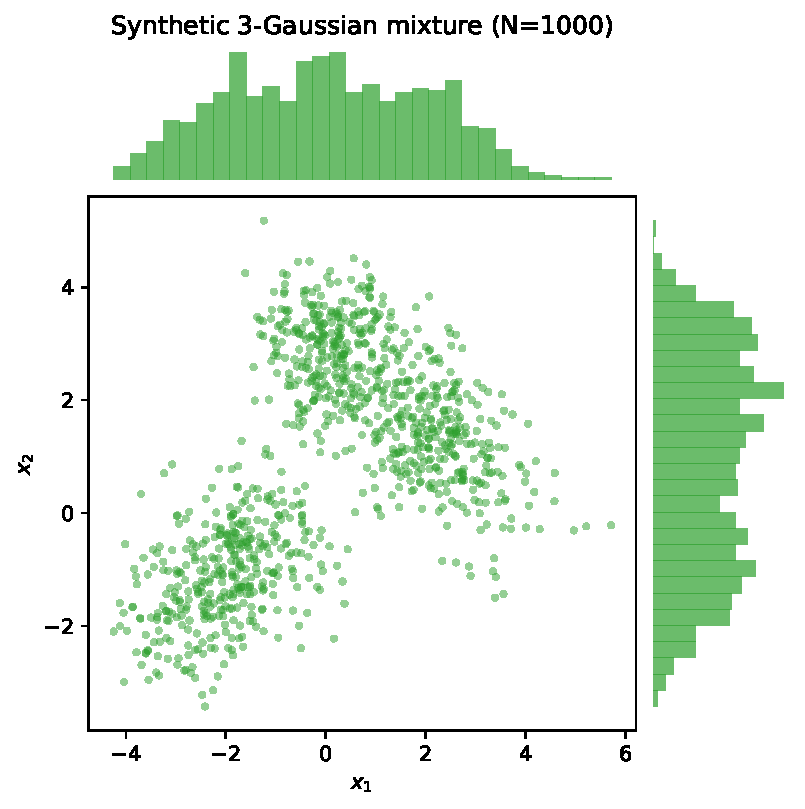
\includegraphics[width=\textwidth]{fig01a_synthetic_scatter.pdf}
    \caption{Synthetic 3-Gaussian mixture.}
  \end{subfigure}\hfill
  \begin{subfigure}{0.48\textwidth}
    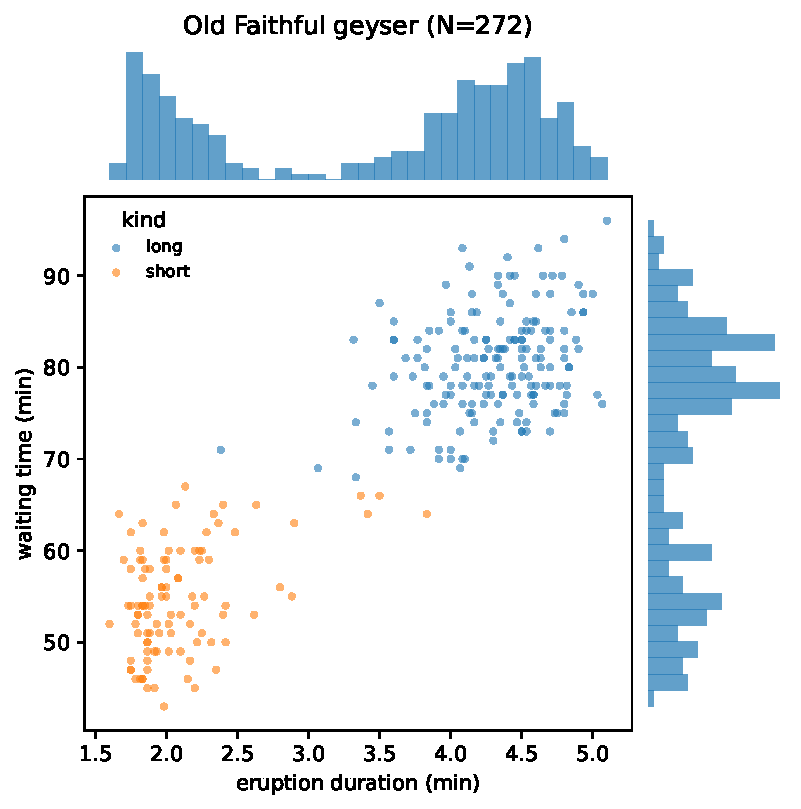
\includegraphics[width=\textwidth]{fig01b_faithful_scatter.pdf}
    \caption{Old Faithful geyser.}
  \end{subfigure}
  \caption{The two datasets with marginal histograms.}
  \label{fig:scatter}
\end{figure}

\subsection{Accuracy on synthetic data (4.1)}
Table~\ref{tab:synthetic} reports ISE and held-out log-likelihood over 20 seeds.
The GMM is clearly best (its parametric form matches the generative process). The
two non-parametric methods and the PNN form a close second tier; crucially the
\textbf{PNN tracks the Parzen window almost exactly} (ISE $0.0032$ vs.\ $0.0033$),
confirming that it has learned to reproduce its teacher. The qualitative picture
is the same: Figure~\ref{fig:heat2d} shows the PNN heatmap is visually
indistinguishable from Parzen, the GMM is smoothest, and $k$-NN is the noisiest.
Figure~\ref{fig:curves1d} shows the analogous 1D density curves.

\begin{table}[t]
\centering
\caption{Synthetic 2D accuracy over 20 seeds (mean $\pm$ std). ISE: lower is
better; log-likelihood: higher is better. Best in \textbf{bold}.}
\label{tab:synthetic}
\begin{tabular}{lcc}
\toprule
Method & ISE $\downarrow$ & held-out log-likelihood $\uparrow$ \\
\midrule
Parzen & $0.00330 \pm 0.00028$ & $-3.539 \pm 0.013$ \\
$k$-NN & $0.00295 \pm 0.00029$ & $-3.576 \pm 0.015$ \\
\textbf{GMM} & $\mathbf{0.00057 \pm 0.00020}$ & $\mathbf{-3.465 \pm 0.018}$ \\
PNN & $0.00324 \pm 0.00028$ & $-3.547 \pm 0.014$ \\
\bottomrule
\end{tabular}
\end{table}

\begin{figure}[t]
  \centering
  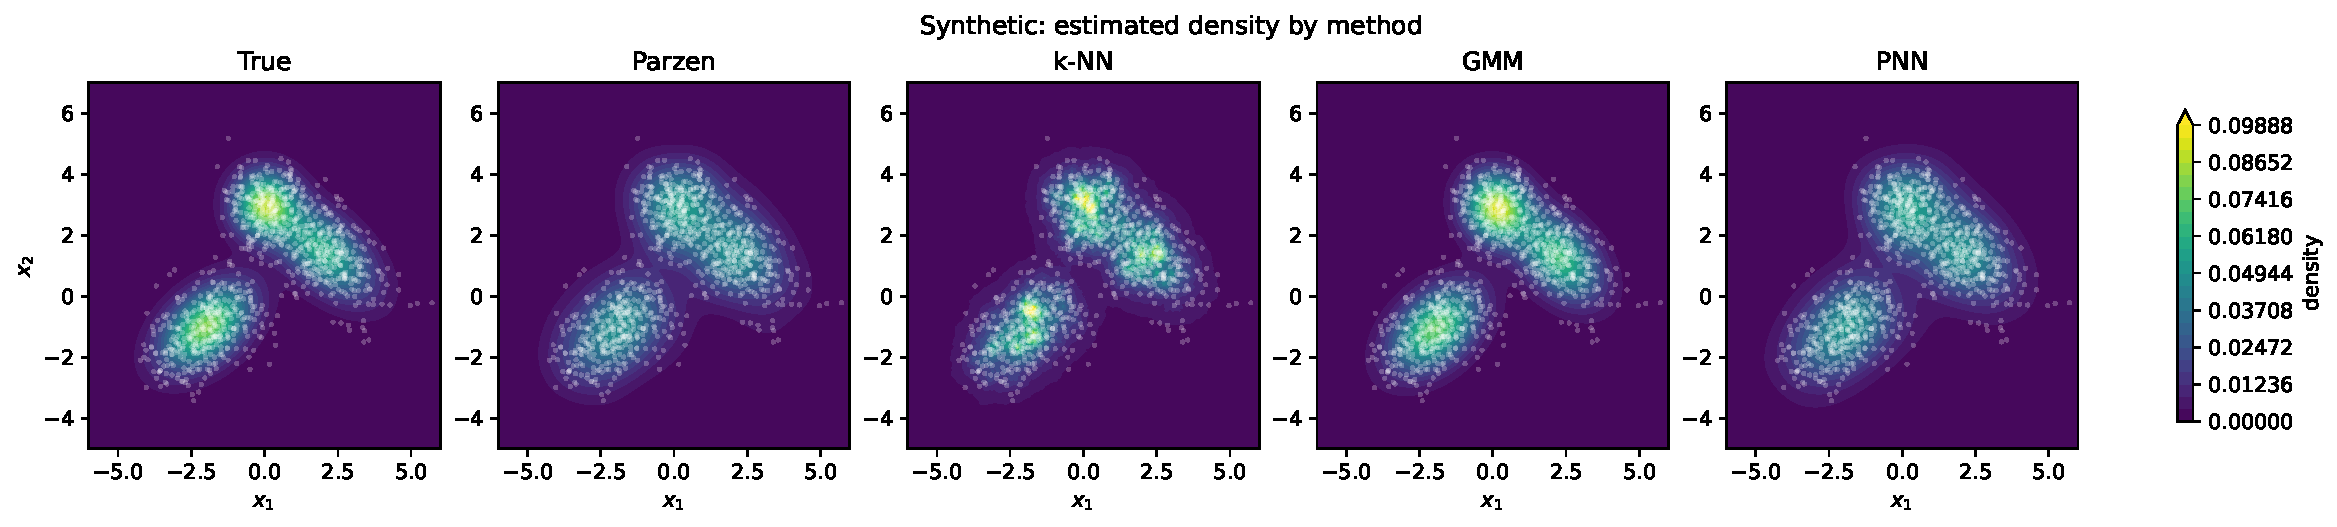
\includegraphics[width=\textwidth]{fig03a_synthetic_heatmaps.pdf}
  \caption{Estimated density on the synthetic data. The PNN reproduces the
  Parzen estimate; the GMM is smoothest; $k$-NN is the noisiest.}
  \label{fig:heat2d}
\end{figure}

\begin{figure}[t]
  \centering
  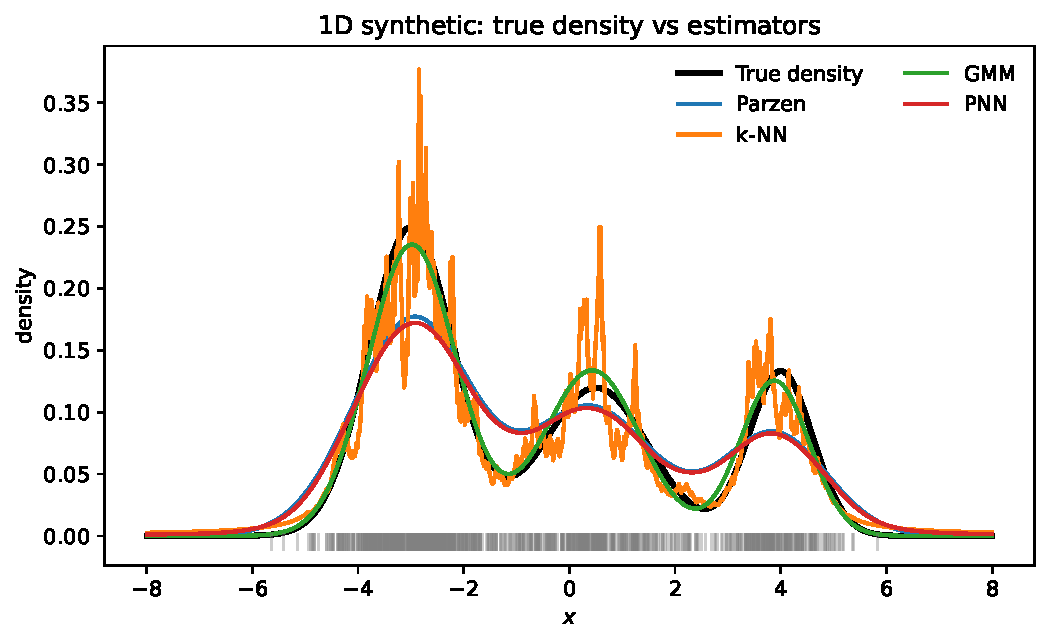
\includegraphics[width=0.85\textwidth]{fig02_1d_density_curves.pdf}
  \caption{1D synthetic data: true density versus each estimator.}
  \label{fig:curves1d}
\end{figure}

\subsection{Accuracy on Old Faithful (4.2)}
Table~\ref{tab:faithful} gives the 10-fold cross-validated log-likelihood. The
ranking is preserved: GMM best, then the Parzen/PNN pair, then $k$-NN. As a
correctness check, the GMM recovers the published bimodal structure: its fitted
waiting-time component means are $54.5$ and $80.0$ minutes, against the published
values $54.6$ and $80.1$~\cite{azzalini1990} (absolute error $\approx 0.13$).
The estimated densities are shown in Figure~\ref{fig:heatfaithful}.

\begin{table}[t]
\centering
\caption{Old Faithful held-out log-likelihood (10-fold CV, mean $\pm$ std).}
\label{tab:faithful}
\begin{tabular}{lc}
\toprule
Method & log-likelihood $\uparrow$ \\
\midrule
Parzen & $-4.467 \pm 0.090$ \\
$k$-NN & $-5.000 \pm 0.260$ \\
\textbf{GMM} & $\mathbf{-4.203 \pm 0.173}$ \\
PNN & $-4.462 \pm 0.089$ \\
\bottomrule
\end{tabular}
\end{table}

\begin{figure}[t]
  \centering
  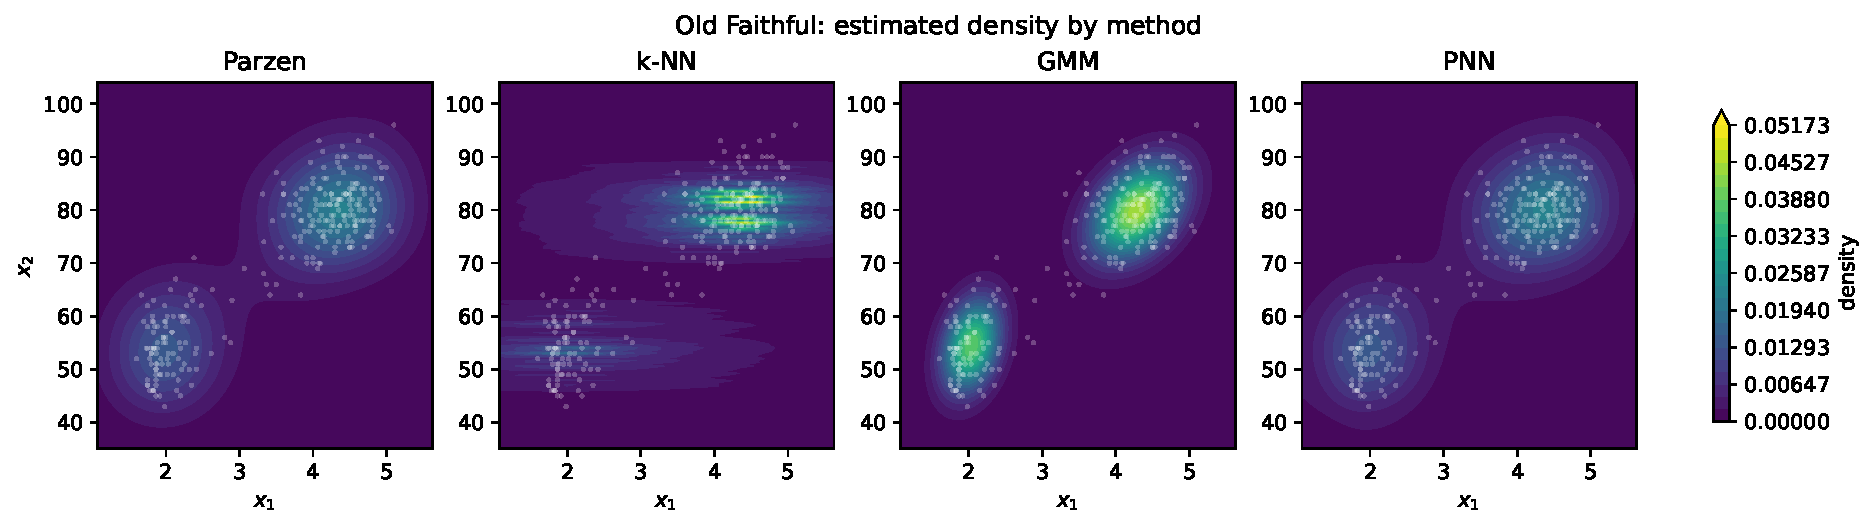
\includegraphics[width=0.95\textwidth]{fig03b_faithful_heatmaps.pdf}
  \caption{Estimated density on Old Faithful (true density unknown).}
  \label{fig:heatfaithful}
\end{figure}

\subsection{Query-time scalability (4.3)}
This is the PNN's headline advantage. Table~\ref{tab:timing} and
Figure~\ref{fig:timing} report the time to score 2000 query points as $N$ grows.
Parzen and $k$-NN scale linearly with $N$ (each query sums or searches over all
training points), whereas the GMM and the PNN are essentially constant. At
$N=5000$ the PNN scores the query set about $300\times$ faster than Parzen while,
as shown above, matching its accuracy.

\begin{table}[t]
\centering
\caption{Query time (milliseconds) to score 2000 points vs.\ training size $N$.}
\label{tab:timing}
\begin{tabular}{lcccc}
\toprule
$N$ & Parzen & $k$-NN & GMM & PNN \\
\midrule
100  & $1.91$  & $0.95$ & $0.59$ & $0.37$ \\
500  & $6.62$  & $3.85$ & $0.52$ & $0.41$ \\
1000 & $18.05$ & $9.33$ & $0.55$ & $0.42$ \\
5000 & $112.7$ & $56.1$ & $0.60$ & $0.38$ \\
\bottomrule
\end{tabular}
\end{table}

\begin{figure}[t]
  \centering
  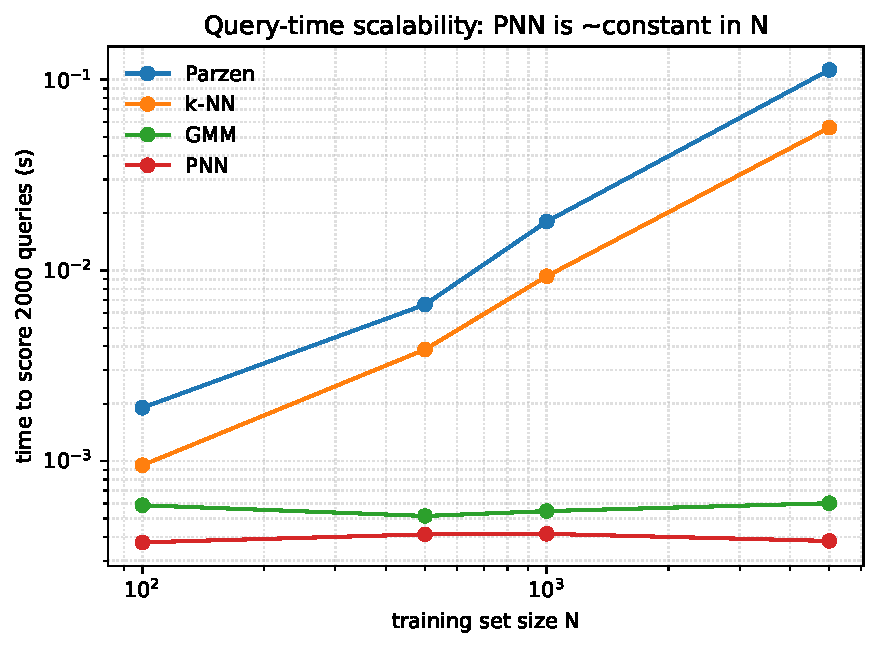
\includegraphics[width=0.7\textwidth]{fig06_query_time_vs_N.pdf}
  \caption{Query time vs.\ $N$ (log--log). Parzen and $k$-NN grow linearly;
  GMM and PNN are $\sim$constant.}
  \label{fig:timing}
\end{figure}

\subsection{Statistical significance (4.4)}
We test every pair of methods with the Wilcoxon signed-rank test (paired,
non-parametric) on the per-seed and per-fold metric values, correcting for the
multiple comparisons with the Holm--Bonferroni procedure. Table~\ref{tab:stats}
reports the Holm-adjusted $p$-values. On the synthetic data all differences are
significant. On Old Faithful all pairs are significant \emph{except
Parzen vs.\ PNN} ($p=0.32$): statistically, the PNN is indistinguishable from
the Parzen window it approximates, which is precisely the desired result given
its query-time advantage.

\begin{table}[t]
\centering
\caption{Holm-adjusted Wilcoxon $p$-values for each method pair.
$^{*}$ significant at $\alpha=0.05$.}
\label{tab:stats}
\begin{tabular}{lccc}
\toprule
Pair & Synthetic ISE & Synthetic log-lik & Old Faithful log-lik \\
\midrule
Parzen vs.\ $k$-NN & $<10^{-4\,*}$ & $<10^{-4\,*}$ & $0.012^{*}$ \\
Parzen vs.\ GMM    & $<10^{-4\,*}$ & $<10^{-4\,*}$ & $0.012^{*}$ \\
Parzen vs.\ PNN    & $0.0006^{*}$  & $0.0027^{*}$  & $0.323$ \\
$k$-NN vs.\ GMM    & $<10^{-4\,*}$ & $<10^{-4\,*}$ & $0.012^{*}$ \\
$k$-NN vs.\ PNN    & $0.0001^{*}$  & $<10^{-4\,*}$ & $0.012^{*}$ \\
GMM vs.\ PNN       & $<10^{-4\,*}$ & $<10^{-4\,*}$ & $0.012^{*}$ \\
\bottomrule
\end{tabular}
\end{table}

\subsection{Bandwidth and $k$ sensitivity (4.5)}
Figure~\ref{fig:sweeps} sweeps the Parzen bandwidth $h$ and the $k$-NN neighbour
count $k$. Both show the classic bias--variance trade-off: too small ($h$ narrow,
$k$ small) gives a spiky, overfit estimate with poor ISE and log-likelihood; too
large oversmooths. The optima sit in the expected middle range, motivating the
cross-validated bandwidth selection we provide.

\begin{figure}[t]
  \centering
  \begin{subfigure}{0.49\textwidth}
    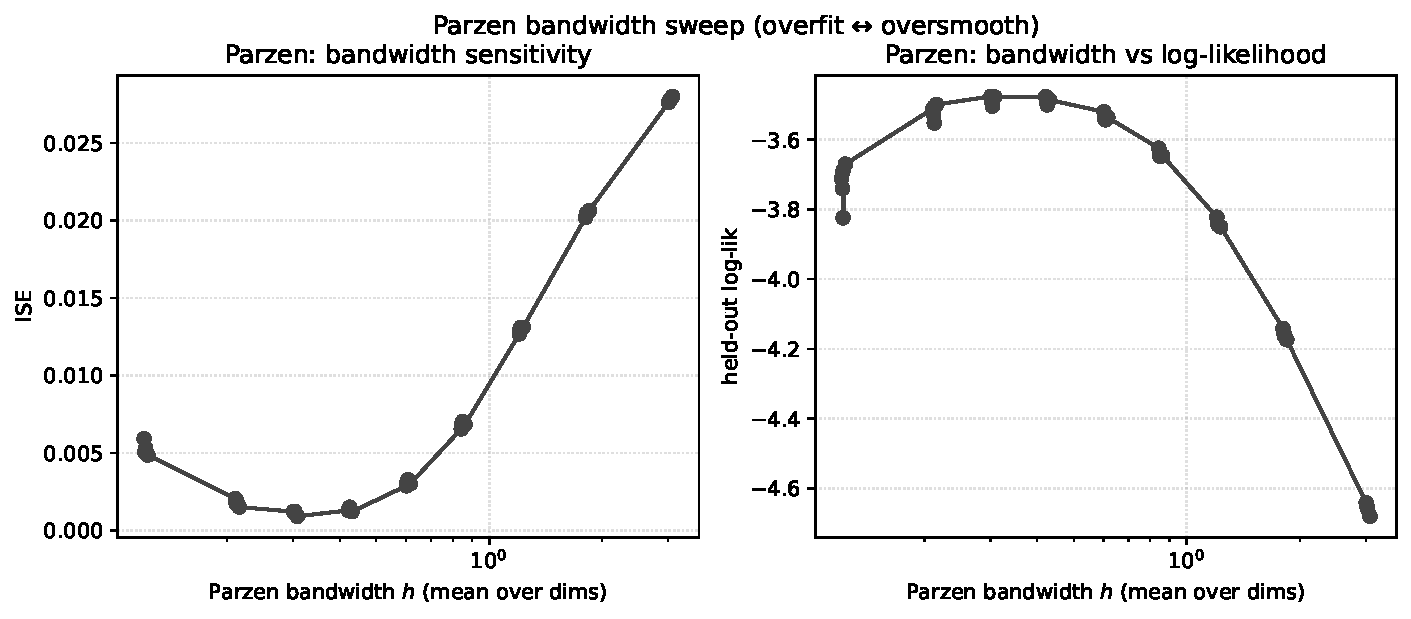
\includegraphics[width=\textwidth]{fig07a_parzen_bandwidth_sweep.pdf}
    \caption{Parzen bandwidth $h$.}
  \end{subfigure}\hfill
  \begin{subfigure}{0.49\textwidth}
    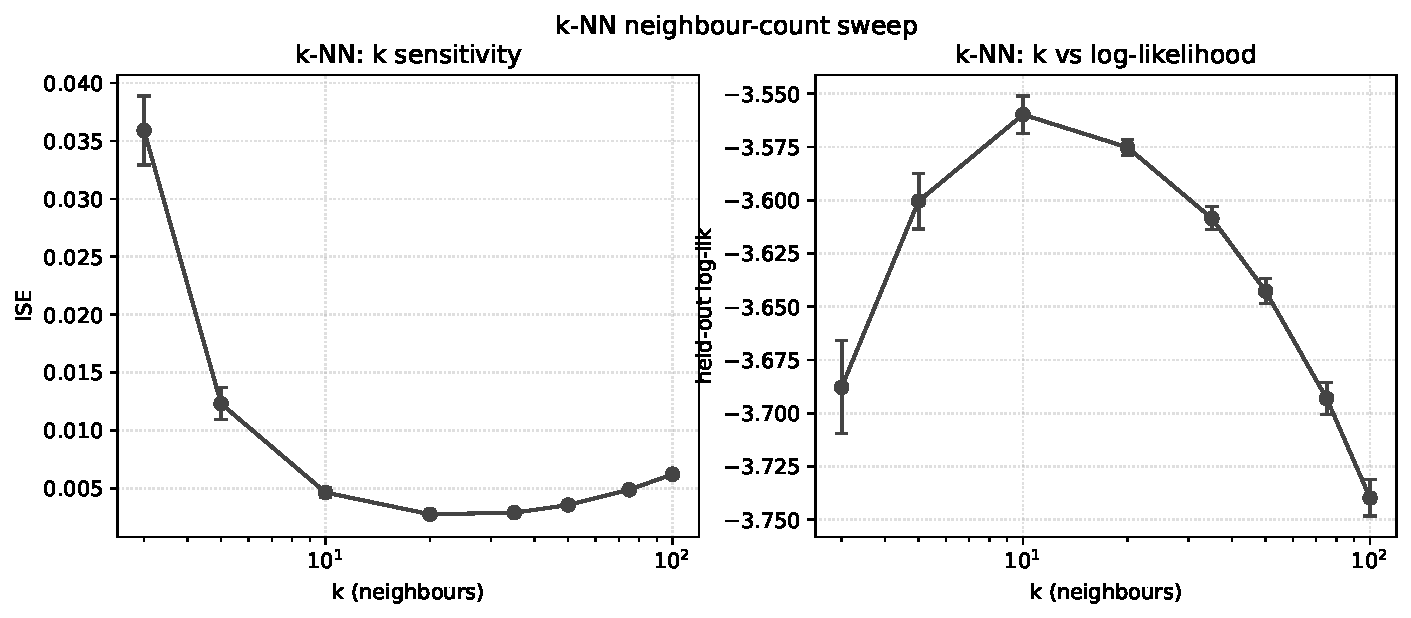
\includegraphics[width=\textwidth]{fig07b_knn_k_sweep.pdf}
    \caption{$k$-NN neighbour count $k$.}
  \end{subfigure}
  \caption{Hyperparameter sensitivity (overfit $\leftrightarrow$ oversmooth).}
  \label{fig:sweeps}
\end{figure}

\subsection{PNN soft-constraint ablation (4.6)}
Finally we ablate the unit-integral penalty (Table~\ref{tab:ablation},
Figure~\ref{fig:ablation}). Without the constraint the learned density integrates
to $1.045$ on average; with it, to $1.007$ --- a clear improvement in
probabilistic validity --- while ISE and log-likelihood are statistically
unchanged. The soft constraint therefore buys Kolmogorov-axiom compliance for
free, supporting Trentin's argument~\cite{trentin2018soft}.

\begin{table}[t]
\centering
\caption{PNN with vs.\ without the unit-integral soft constraint (10 seeds).}
\label{tab:ablation}
\begin{tabular}{lccc}
\toprule
Variant & ISE $\downarrow$ & log-lik $\uparrow$ & $\int f_\theta$ (target 1) \\
\midrule
without constraint & $0.00324 \pm 0.00030$ & $-3.533 \pm 0.016$ & $1.045 \pm 0.014$ \\
with constraint    & $0.00312 \pm 0.00026$ & $-3.543 \pm 0.011$ & $\mathbf{1.007 \pm 0.011}$ \\
\bottomrule
\end{tabular}
\end{table}

\begin{figure}[t]
  \centering
  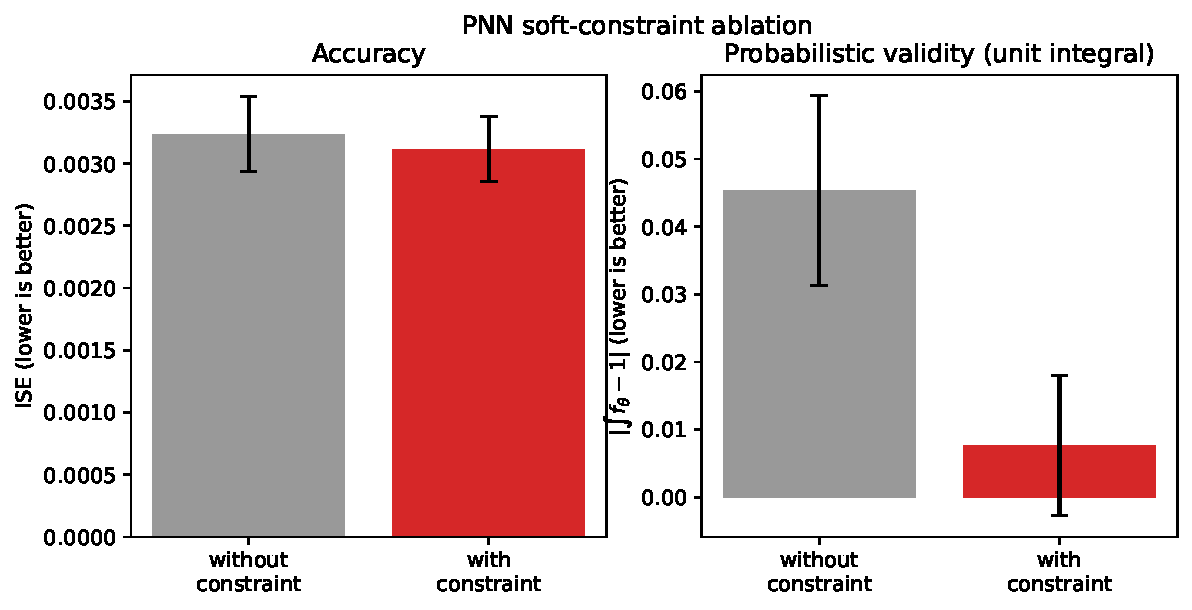
\includegraphics[width=0.7\textwidth]{fig09_pnn_ablation.pdf}
  \caption{The soft constraint pulls the integral towards 1 at no accuracy cost.}
  \label{fig:ablation}
\end{figure}

% ============================================================================
\section{Discussion}
% ============================================================================
The results form a coherent picture. The \textbf{GMM} wins on accuracy because
both datasets really are (close to) Gaussian mixtures --- a reminder that a
correct parametric assumption is hard to beat, but also a caveat: this advantage
would vanish on data the GMM cannot represent. The \textbf{non-parametric}
estimators are assumption-light and competitive in accuracy but pay for it at
query time, where their cost grows linearly with the training set. The
\textbf{PNN} is the interesting middle ground: it inherits the Parzen window's
accuracy (statistically indistinguishable on Old Faithful) while amortising the
per-query cost into a one-off training phase, giving roughly constant-time
evaluation. The soft integral constraint makes its output a legitimate density
without harming the fit. We also note the practical lesson that the constraint
weight must be made scale-aware, otherwise it fails to transfer between 1D and 2D
problems.

\textbf{Limitations.} We deliberately stay in 1--2 dimensions; all of these
methods suffer the curse of dimensionality, which is itself the point rather than
a flaw to engineer around. The PNN's training cost grows with $N$ (it must
compute the Parzen target), so its advantage is realised only when the model is
queried far more often than it is trained --- which is the common deployment
regime.

% ============================================================================
\section{Conclusion}
% ============================================================================
We compared four density estimators under a reproducible protocol with ISE,
held-out log-likelihood, a scalability benchmark, and rigorous significance
testing. The GMM is most accurate when its assumptions hold; the Parzen window
and $k$-NN are flexible but slow at query time; and the Parzen Neural Network
recovers the Parzen estimate's accuracy while evaluating in constant time and
remaining a valid probability density through a soft Kolmogorov-axiom constraint.
This reproduces, on independent data and implementation, the central finding of
Trentin and Gori.

% ============================================================================
\section*{Author Contributions}
% ============================================================================
\noindent
\textbf{Leonid Vasilev (163880):} non-parametric estimators (Parzen window and
$k$-NN density), the metrics and numerical-integration module, and the
validation tests.\\
\textbf{Akbar Hasanov (167789):} the Parzen Neural Network (architecture,
soft-constrained training, scale-aware loss), the experiment orchestration and
the reproducible pipeline.\\
\textbf{Basel Altamimi (169559):} the Gaussian Mixture Model and BIC selection,
the statistical analysis (Wilcoxon/Holm), the dataset handling, and the figures.\\
All authors contributed to the experimental design and to writing this report.

% ============================================================================
\begin{thebibliography}{9}
% ============================================================================
\bibitem{trentin2001parzen}
E.~Trentin and M.~Gori.
\emph{Parzen Neural Networks}. Course material, University of Siena.

\bibitem{trentin2018soft}
E.~Trentin et al.
\emph{Soft-constrained artificial neural networks satisfying the Kolmogorov
axioms of probability}. Course material, University of Siena.

\bibitem{parzen1962}
E.~Parzen.
\emph{On estimation of a probability density function and mode}.
The Annals of Mathematical Statistics, 33(3):1065--1076, 1962.

\bibitem{duda2001}
R.~O.~Duda, P.~E.~Hart, and D.~G.~Stork.
\emph{Pattern Classification}, 2nd ed. Wiley, 2001.

\bibitem{bishop2006}
C.~M.~Bishop.
\emph{Pattern Recognition and Machine Learning}. Springer, 2006.

\bibitem{silverman1986}
B.~W.~Silverman.
\emph{Density Estimation for Statistics and Data Analysis}.
Chapman \& Hall, 1986.

\bibitem{azzalini1990}
A.~Azzalini and A.~W.~Bowman.
\emph{A look at some data on the Old Faithful geyser}.
Applied Statistics, 39(3):357--365, 1990.

\bibitem{pedregosa2011}
F.~Pedregosa et al.
\emph{Scikit-learn: Machine Learning in Python}.
Journal of Machine Learning Research, 12:2825--2830, 2011.

\bibitem{paszke2019}
A.~Paszke et al.
\emph{PyTorch: An Imperative Style, High-Performance Deep Learning Library}.
NeurIPS, 2019.
\end{thebibliography}

\end{document}
